% \AtBeginSection[]{
% 	\begin{frame}
% 		\frametitle{}
% 		\tableofcontents[currentsection]
% 	\end{frame}
% }

%%%%%%%%%%%%%%%%%%%%%%%%%%%%%%%%%%%%
 
 \section{Formal model and simulation}

        \subsection{Formal model for \textquote{cyber-attackers vs. cyber-defenders}}
        
 	\begin{frame}{Formal model for \textquote{cyber-attackers vs. cyber-defenders}}
		{Decentralized Partially Observable Markov Decision Process}

            Receiving last observations and reward from previous iteration and choosing next action.

            \begin{figure}
                \centering
                \includesvg[width=1.05\textwidth]{figures/model_illustration_1.svg}
            \end{figure}
  
	\end{frame}

 	\begin{frame}{Formal model for \textquote{cyber-attackers vs. cyber-defenders}}
		{Decentralized Partially Observable Markov Decision Process}

            Applying chosen actions to change environment properties.

            \begin{figure}
                \centering
                \includesvg[width=1.05\textwidth]{figures/model_illustration_2.svg}
            \end{figure}
  
	\end{frame}

 	\begin{frame}{Formal model for \textquote{cyber-attackers vs. cyber-defenders}}
		{Decentralized Partially Observable Markov Decision Process}

            Next iteration: receiving new observations and choosing action\dots

            \begin{figure}
                \centering
                \includesvg[width=0.65\textwidth]{figures/model_illustration_3.svg}
            \end{figure}

            \vspace{-0.1cm}

            Ends when maximum iteration number or attack goal is reached.
  
	\end{frame}

        \subsection{Simulation implementation}
	% \begin{frame}{Simulation implementation}
 %            {Available simulation works}

 %            \begin{block}{Potential \textquote{ready to use} simulators}
 %                \begin{itemize}
 %                    \item \textit{NeSSi2}~\cite{DGrunewald2011}: an agent-based simulation platform aiming to model only packet-level description of a networked system and the effects of DDoS attacks;
 %                    \item Kotenko et al.~\cite{IKotenko2007} relies on \textit{OMNet++}~\cite{Varga2010} to model and simulate cooperative cyber-defense agents against network attacks.
 %                \end{itemize}
 %            \end{block}
            
 %            However, among these, none can fully meet both the consideration of a multi-agent cyber environment for a Dec-POMDP model.

 %            \begin{block}{Tools towards implementing}
 %                \begin{itemize}
 %                    \item Extending discrete-event simulators such as \textit{CYST}\cite{drasar_session-level_2020} or \textit{CyberBattleSim}~\cite{cyberbattlesim} for multi-agent context
 %                    \item Using \textit{PettingZoo}~\cite{jk2020} which is a platform designed to implement a Dec-POMDP model
 %                \end{itemize}
 %            \end{block}
      
	% \end{frame}


        \begin{frame}{Model implementation as a simulation}
            {}

            No available simulator fully meet both the consideration of a multi-agent cyber environment for a Dec-POMDP model but\dots

            \begin{itemize}
                \item Extending discrete-event simulators such as \textit{CYST}\cite{drasar_session-level_2020} or \textit{CyberBattleSim}~\cite{cyberbattlesim} for multi-agent context
                \item Using \textit{PettingZoo}~\cite{jk2020} which is a platform designed to implement a Dec-POMDP model
            \end{itemize}

            \

            \begin{block}{Multi Cyber Agent Simulator (MCAS)~\cite{MCASWebsite}}

                \begin{itemize}
                    \item Loading/saving a scenario file describing the nodes properties, actions of the environment and the defined agents with their behaviors;
                    \item Executing the agents of this environment in turn-by-turn mode via the API or graphical interface;
                    \item Viewing the environment and metrics.
                \end{itemize}

            \end{block}

        \end{frame}

        
        \begin{frame}{Model implementation as a simulation}
            {}

            \begin{figure}
                \centering
                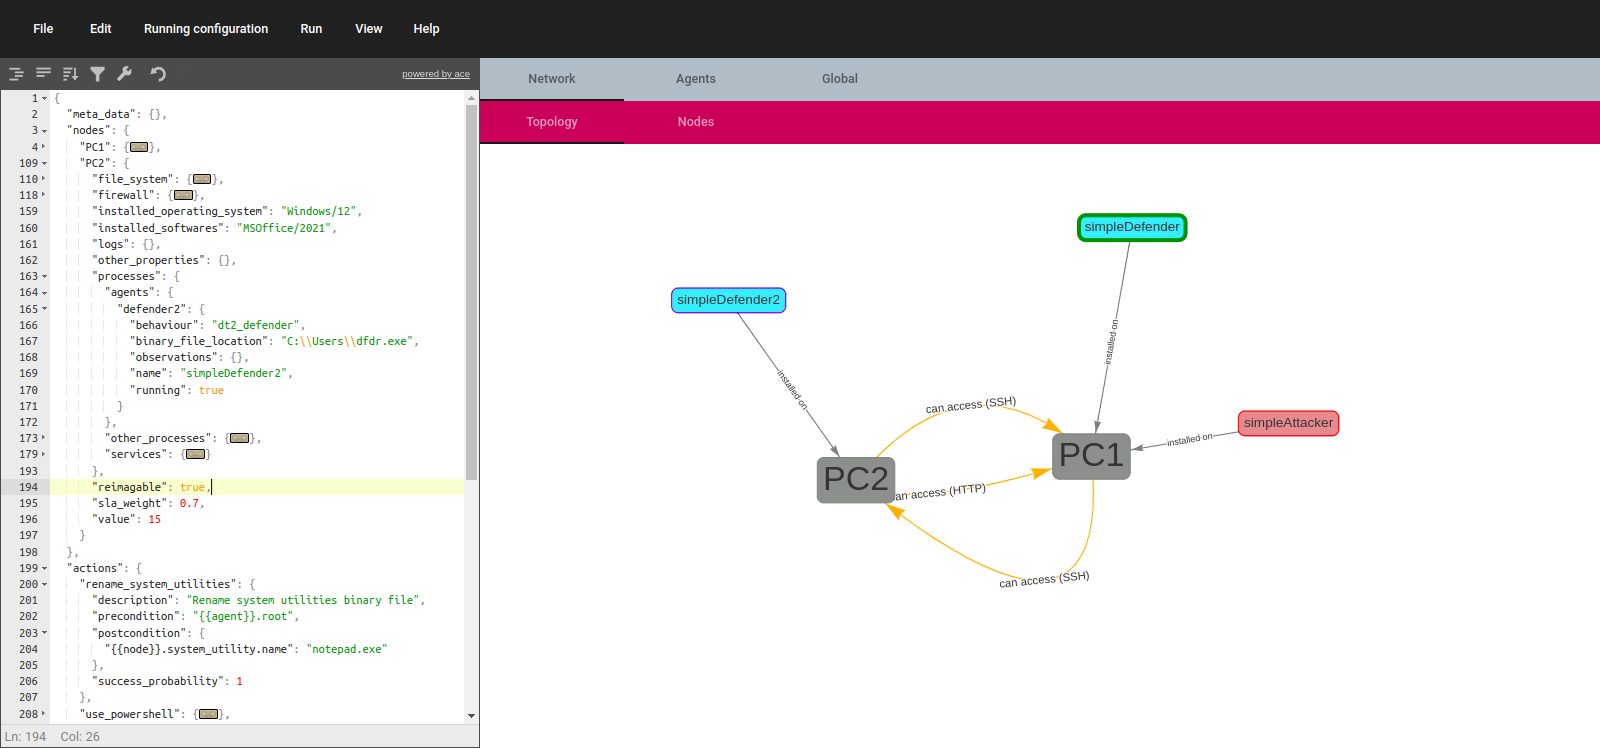
\includegraphics[width=0.95\textwidth]{figures/interface_MCAS.png}
                \caption{Overview of the MCAS interface}
                \label{fig:interface_simulateur}
            \end{figure}
        
        \end{frame}

        % \begin{frame}{Simulation implementation}
        %     {MCAS: Multi Cyber Agent Simulator}
        
        %     \begin{center}
        %             \embedvideo{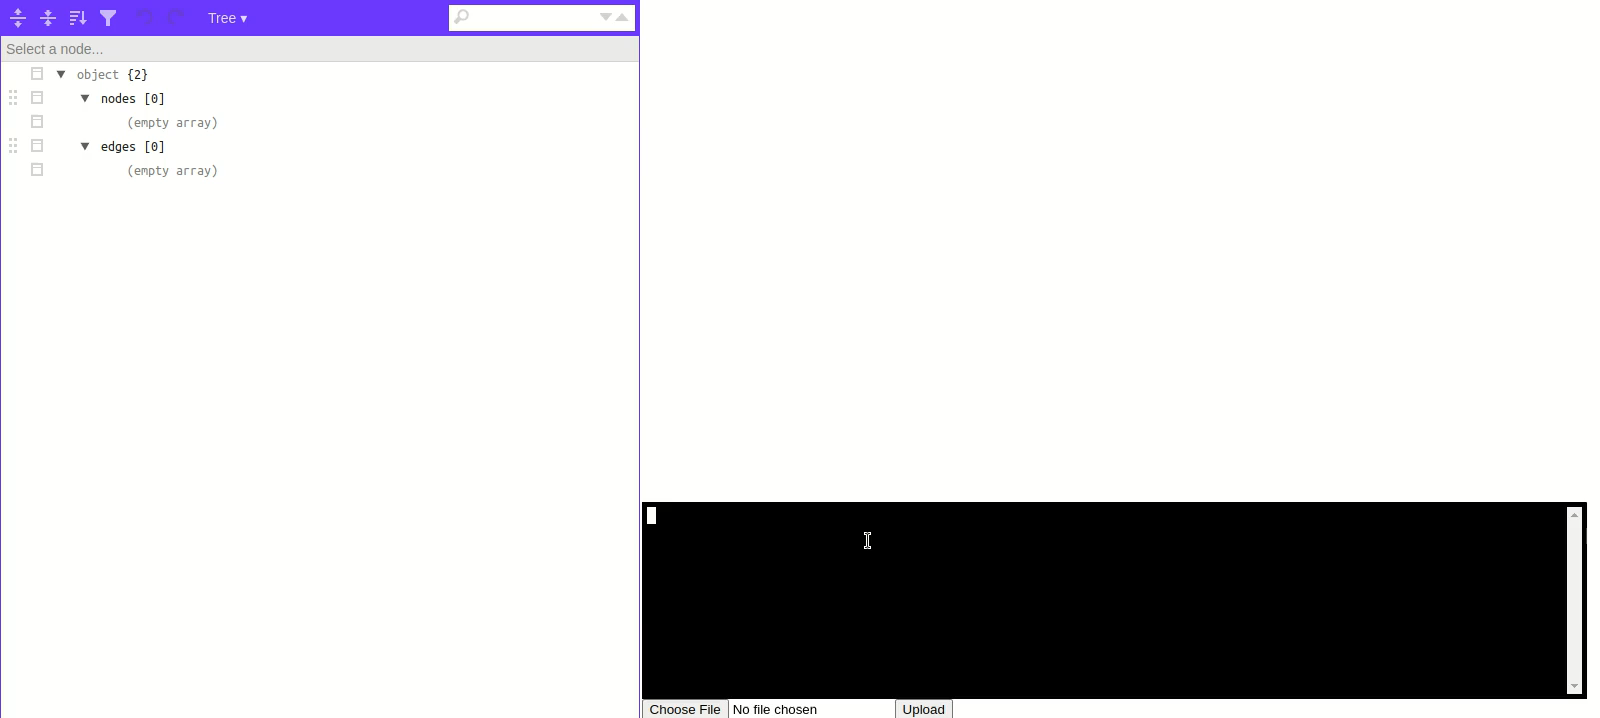
\includegraphics[width=\textwidth]{videos/thumbnail.png}}{videos/mcas_presentation.mp4}
        %     \end{center}
            
        % \end{frame}

 
	% \subsection{Attack/Defense scenarios integration}
	% \begin{frame}{Attack/Defense scenarios integration}
 %            {Integration approach}

 %            A high-level manual approach to integrate MITRE ATT\&CK information as an AD tree to formalize actions to be played in a scenario through the simulator.

 %            \begin{enumerate}
            
 %                \item Identify relevant tactics and techniques and procedures from MITRE ATT\&CK for an Advanced Persistent Threat (APT);
                
 %                \item Link tactics together and associated techniques, sub-techniques and procedures to create a scenario that describes how the APT group could attack the networked system;
            
 %                \item Establish an AD tree with tactics as top action goals while techniques, sub-techniques and procedures are in the lower part of the tree;
            
 %                \item Decorate the attack nodes with the MITRE ATT\&CK detection and mitigations.
                
 %            \end{enumerate}

        % \end{frame}

